\section{Numerical method and verification}
\label{sec:numerical}

\subsection{MRT-lattice Boltzmann scheme}
\label{subsec:mrt}

The solver employs a D2Q9 multiple-relaxation-time lattice Boltzmann method. The distribution functions $f_i$ are discretized on a nine-velocity square lattice. In the MRT formulation, the populations are transformed to the moment space, collided with a diagonal relaxation matrix, and transformed back before streaming. The relaxation time $\tau$ is related to the kinematic viscosity through
\begin{equation}
\nu = c_s^2\left(\tau - \tfrac{1}{2}\right)\Delta t,
\end{equation}
where $c_s^2 = 1/3$ for the D2Q9 lattice. The relaxation rates for the non-hydrodynamic moments are chosen following standard MRT practice to enhance numerical stability; only the shear mode uses $\tau$, while the remaining rates are fixed at values appropriate for the low-Mach regime considered here.

The lattice velocity is set from $U=(\tau-\tfrac12)\,Re/(3N)$, so that the target Reynolds number fixes $\tau$ through $Re=UN/\nu_{\mathrm{lat}}$ with $\nu_{\mathrm{lat}}=\tfrac13(\tau-\tfrac12)$. Table~\ref{tab:params} lists the actual $(\tau,U,Ma)$ values for each $Re$ family; the lattice Mach number is not identical across the three Reynolds numbers because $\tau$ is chosen for numerical stability rather than to keep $Ma$ fixed.

\subsection{Wall treatments}
\label{subsec:walls}

\paragraph{Curved bottom wall.}
The bottom boundary combines a staircase solid/fluid mask with Bouzidi interpolated bounce-back~\cite{Bouzidi2001}. The staircase mask classifies a cell as fluid or solid according to whether its centre lies above or below the wall $y_b(x)$, and is used only to decide which nodes are active. The boundary condition itself is not staircase: for every fluid node adjacent to the wall, the lattice link that crosses $y_b(x)$ is intersected analytically and the fractional distance $q$ to the wall is computed; the unknown population is then reconstructed by linear interpolation between the wall and the upstream fluid node, weighted by $q$. This is the standard second-order Bouzidi scheme. The distinction matters for interpretation: the mask defines the active-node set and therefore introduces a grid-dependent representation of the computational domain, whereas the Bouzidi interpolation imposes the no-slip condition at the analytic wall location. The dissipation is evaluated as a volume integral of discrete strain-rate values; its sensitivity to the near-wall gradient treatment is assessed separately in Section~\ref{subsec:robustness}.

\paragraph{Moving lid.}
The lid velocity is imposed using a regularized momentum injection: the top-wall links receive a prescribed momentum consistent with the lid velocity, smoothed near the corners with a smoothstep profile of width $\varepsilon=0.02$. This is not a Zou--He boundary nor a general regularization of the LBM collision operator; it is a link-based momentum forcing that reproduces the prescribed lid velocity while mitigating the corner singularity.

\subsection{Numerical parameter matrix}
\label{subsec:params}

The lattice velocity is set from $U=(\tau-\tfrac12)\,Re/(3N)$, i.e.\ by \emph{diffusive scaling}: $\tau$ (hence $\nu_{\rm lat}$) is fixed per Reynolds number while $U\propto1/N$, so $Ma=U/c_s$ decreases with refinement. Table~\ref{tab:params} lists the actual $(\tau,U,Ma)$ values. At $N=384$ (the production grid) $Ma\simeq0.0226$ ($Re=100$) and $Ma\simeq0.0601$ ($Re=400,1000$); at the coarser test grids the Mach number is larger---$Ma\simeq0.0338$ and $0.0902$ at $N=256$, and $Ma\simeq0.0677$ and $0.1804$ at $N=128$, for $Re=100$ and $Re\ge400$ respectively. Because the resolution study holds $\tau$ fixed at each $Re$, the grid is refined at constant physical viscosity and the comparison legitimately isolates the discretisation; the accompanying change of $Ma$ is a consequence of the diffusive scaling rather than an independent parameter. The study is nevertheless not matched in $Ma$ across Reynolds numbers, and compressibility differences between $Re=100$ and the higher Reynolds numbers are not isolated; the comparison of geometric contrasts remains internal to each Reynolds number, where $Ma$ is fixed. In addition, the fine 19-point Reynolds sweep at $N=128$ ($Re\in[100,1000]$ in steps of $50$) is fully documented in Table~SM.III of the Supplemental Material; for $Re\ge 150$ it maintains $U=5/48\approx0.104167$ ($Ma\approx0.1804$) with $\tau=0.5+40/Re$.

\begin{table}[t]
\centering
\caption{LBM numerical parameters for the three Reynolds-number families at $N=384$. $N$ is the grid resolution, $\tau$ the relaxation time, $U$ the lattice lid velocity, and $Ma=U/c_s$ the lattice Mach number.}
\label{tab:params}
\begin{tabular}{@{}ccccc@{}}
\hline
$Re$ & $N$ & $\tau$ & $U$ & $Ma$ \\
\hline
$100$  & $384$ & $0.65$ & $0.01302$ & $0.0226$ \\
$400$  & $384$ & $0.60$ & $0.03472$ & $0.0601$ \\
$1000$ & $384$ & $0.54$ & $0.03472$ & $0.0601$ \\
\hline
\end{tabular}
\end{table}
\subsection{Convergence criterion}
\label{subsec:convergence}

Each simulation is run until the relative change of the velocity field between successive measurement windows falls below $10^{-8}$. The final iteration count and residual are recorded for every case; all $24$ cases in the $N=384$ main campaign ($N_w=1$, $\alpha\in\{0,0.1\}$) satisfied this criterion, with residuals at or below $9.9\times10^{-9}$. The six supplementary cases extended to $N=512$ ($Re=400$ and $Re=1000$, $n\in\{2,4,6,8\}$, $\alpha=0$) likewise converged, with residuals between $9.86\times10^{-9}$ and $9.98\times10^{-9}$ and iteration counts between $500\,000$ and $1\,202\,000$. Iterative convergence of the discrete solution does not, by itself, establish spatial convergence of the energetic integrals; this distinction is developed in Section~\ref{subsec:resolution}.

\subsection{Numerical verification against the square-cavity benchmark}
\label{subsec:validation}

The square cavity ($A_f=1$, flat bottom) is the standard benchmark of Ghia et al.~\cite{Ghia1982}. Four verifications are reported. First, an \emph{exact} square cavity with a flat bottom and a uniform (non-regularized) lid is run directly at $Re=100$, $400$, and $1000$; the centerline profiles are compared pointwise with the tabulated data of Ghia et al.~\cite{Ghia1982} in Table~\ref{tab:ghia}. Both the horizontal velocity $u$ along the vertical centerline $x=0.5$ and the vertical velocity $v$ along the horizontal centerline $y=0.5$ match the reference to within a few percent of the lid velocity: at $N=256$ the maximum absolute deviations are $0.0062$ and $0.0102$ at $Re=100$, $0.0033$ and $0.0058$ at $Re=400$, and $0.0050$ and $0.0136$ at $Re=1000$ (the latter spectral reference case is that of Botella and Peyret~\cite{Botella1998}). The vertical-velocity error at $Re=400$ is dominated by a single non-monotone tabulated datum at $x=0.9063$ that is commonly treated as anomalous~\cite{Chai2006}; excluding it, $\max|v-v_G|$ is $0.0058$, consistent with the other Reynolds numbers. Second, the campaign includes a near-square case ($n=8$, $\alpha=0$, $A_f=0.9892<1$) that uses the \emph{regularized} production lid, compared with the same benchmark in Fig.~\ref{fig:benchmark}. Using the same interior centerline stations and the same exclusion of the anomalous $Re=400$ datum, its maximum deviations at $N=256$ are $0.0038$ and $0.0054$ at $Re=100$, $0.0035$ and $0.0034$ at $Re=400$, and $0.0046$ and $0.0066$ at $Re=1000$---i.e.\ of the same order as, and in several cases smaller than, the exact-square deviations, despite the regularized lid (which differs from the uniform lid of Ghia et al.\ near the top corners) and the small rounding of the $n=8$ bottom corners. The curved-wall (Bouzidi) treatment and the near-square bottom therefore do not degrade the interior solution. The exact-square test verifies the flat-wall and uniform-lid limits of the solver; the near-square test confirms that the curved-wall treatment does not degrade the interior solution.

Third, to isolate the effect of the regularized lid itself---separately from the curvature and rounded corners of the near-square case---the flat square cavity ($A_f=1$, strictly flat bottom) was recomputed with the \emph{regularized} production lid ($\varepsilon=0.02$) at every Reynolds number and both grids, giving a complete $Re\in\{100,400,1000\}\times N\in\{128,256\}\times\{$uniform$,$regularized$\}$ matrix. The centerline deviations from Ghia et al.\ are essentially unchanged: at $N=256$ the regularized lid gives $0.0062$ and $0.0102$ ($Re=100$), $0.0033$ and $0.0058$ ($Re=400$), and $0.0052$ and $0.0135$ ($Re=1000$) for $\max|u-u_G|$ and $\max|v-v_G|$, against $0.0062/0.0102$, $0.0033/0.0058$, and $0.0050/0.0136$ for the uniform lid---a change of at most $2\times10^{-4}$ on the finest grid. The largest difference anywhere in the matrix is $5.5\times10^{-4}$ on the coarsest grid ($Re=1000$, $N=128$), and the profiles are pointwise within the same tolerance (the full matrix is tabulated in Table~SM.VI of the Supplemental Material). The corner regularization of the lid therefore does not measurably alter the interior flow on a flat geometry; it only removes the corner singularity. This addresses the possible concern that the production lid could bias the bulk solution relative to the standard benchmark.

Fourth, and most directly relevant to the energetic claims, a conforming Taylor--Hood finite-element solver (P2 velocity / P1 pressure, Picard linearisation) was used to recompute the primary contrast $I_D(2,4)$ at $Re=400$, $\alpha=0$ on the \emph{same} superelliptic geometry (identical wall function and fluid area $A_f=0.892699$) and with the \emph{same} regularized lid profile: the prescribed top-boundary velocity reproduces the production cubic-smoothstep lid regularization of width $\varepsilon=0.02$, so the two solvers share the wall geometry, the lid boundary condition, and the definitions of the energetic integrals. All finite-element energetics are evaluated \emph{natively}: the strain-rate, lid-power, and kinetic-energy integrals are taken element-wise from the finite-element velocity field, with no projection and no lattice-Boltzmann wall-gradient model. The native energy balance of the finite-element solution closes to $0.01\%$ on its finest mesh ($P^*=D^*$ to $0.01\%$, and remains within $0.22\%$ over all three FEM meshes; Table~SM.VII of the Supplemental Material), which serves as an internal check of energetic consistency. This near-exact FEM balance closure contrasts with the lattice-Boltzmann discrete calculations, where the global energy defect $|P^*-D^*|/D^*$ is of order $2\%$ on the $N=384$ production grid (reaching up to $2.17\%$, or $\approx 2.2\%$ at most over all production runs; Table~SM.XI of the Supplemental Material), stemming from the discrete resolution of the high-shear lid boundary layer. As shown below, this defect is nearly identical between paired geometries at the same resolution and therefore largely cancels in the differential contrasts ($I_P \approx I_D$). On the finest grids of each solver (FEM $nx=ny=256$, MRT-LBM $N=384$) the absolute n$=2$ levels agree to $1$--$4\%$ ($K^*$: $+1.1\%$, $D^*$: $+2.0\%$, $P^*$: $+4.1\%$), and the three contrasts agree to within $0.02$ percentage point ($I_K$: $0.019$ pt, $I_P$: $0.008$ pt, $I_D$: $0.002$ pt; Table~\ref{tab:femxcheck} and Fig.~\ref{fig:femxcheck}). The dissipation contrast is the most cleanly reproduced: the finite-element sequence $I_D(2,4)=+0.346\%$ ($nx=64$), $+0.332\%$ ($nx=128$), $+0.323\%$ ($nx=256$) is monotone and approaches the lattice-Boltzmann value $+0.325\%$ at $N=384$. The proximity on the finest grids ($0.002$ pt) is encouraging but is a consistency check, not a convergence proof: the finite-element variation across its own three meshes ($0.023$ pt, from $+0.346\%$ to $+0.323\%$) is larger than the final FEM--LBM gap, so the calculation does not by itself demonstrate that the finite-element estimate converges to the lattice-Boltzmann one. The larger absolute $P^*$ offset reflects the rougher resolution of the lid shear layer at $N=384$ together with the residual $2\%$ lattice-Boltzmann power--dissipation imbalance there; it cancels in the paired contrast, as the internal-consistency argument of Section~\ref{subsec:resolution} predicts. The finite-element cross-check therefore corroborates the contrast (to $\lesssim0.02$ pt) and, once each solver is taken at its own finest grid, the absolute dissipation (to $2\%$); it is reported as an independent-solver consistency check, not as a second convergence study. The FEM--LBM comparison is therefore reported strictly as a cross-solver consistency check at $Re = 400$, never as a convergence proof for either solver.

The same solver was run at $Re=1000$, where the check is more informative because the contrast is larger. Restricted to its native element-wise diagnostics it gives $I_D(2,4)=+0.716\%$ at $nx=64$ and $+0.598\%$ at $nx=128$, against $+0.5909\%$ on the lattice-Boltzmann production grid $N=384$: the finer mesh differs by $0.008$ percentage point, or $1.3\%$ in relative terms, and the native finite-element sequence moves toward the lattice-Boltzmann value under refinement. The LBM-grid-projected finite-element contrasts are $+32.6\%$ ($nx=64$) and $+11.8\%$ ($nx=128$) and are not used: projecting the finite-element solution onto the coarser lattice under-resolves the lid shear layer at this Reynolds number. The same projection is already unreliable at $Re=400$, where it yields $+6.1\%$ at $nx=64$ and $+2.0\%$ on the mesh used for the finest native value, against $+0.323\%$ natively. All finite-element--lattice-Boltzmann comparisons in this work therefore use native element-wise integrals.

This verification supports the correctness of the bulk fluid solver and of the curved-wall treatment. The energetic integrals are volume integrals of the stress tensor, so their resolution sensitivity is examined separately in Section~\ref{subsec:resolution}.

\begin{table}[t]
\centering
\caption{Independent-solver cross-validation of the primary contrast $(2,4)$ at $Re=400$, $\alpha=0$: Taylor--Hood finite-element method (P2/P1) \emph{vs.}\ the MRT-LBM, on the identical superelliptic geometry. The comparison is made on the finest grids of each solver (FEM $nx=ny=256$, MRT-LBM $N=384$). All FEM entries are \emph{native}: the strain-rate, lid-power, and kinetic-energy integrals are evaluated element-wise from the finite-element velocity field, without projection. The upper block gives the absolute $n=2$ reference values together with the FEM--LBM \emph{relative} difference (in percent); the lower block gives the geometric contrast $I(2,4)$, whose FEM--LBM difference is expressed in percentage points (pt). The finite-element native energy balance closes to $0.01\%$ on $nx=256$ (and within $0.22\%$ across all FEM meshes). The FEM--LBM contrast differences $\Delta$ (in pt) are computed from the unrounded solver outputs, not from the displayed three-decimal contrasts.}
\label{tab:femxcheck}
\small
\begin{tabular}{@{}lcccc@{}}
\toprule
Quantity & FEM & MRT-LBM & $\Delta_{\rm rel}$ [\%] & $\Delta$ [pt] \\
\midrule
$K^*$ ($n=2$), native  & $0.040440$ & $0.040011$ & $+1.1$ & --- \\
$P^*$ ($n=2$), native  & $23.899$   & $22.954$   & $+4.1$ & --- \\
$D^*$ ($n=2$), native  & $23.896$   & $23.432$   & $+2.0$ & --- \\
$D^*$ ($n=4$), native  & $23.973$   & $23.508$   & $+2.0$ & --- \\
\midrule
$I_{K}(2,4)$ [\%]      & $+0.752$   & $+0.771$   & --- & $0.019$ \\
$I_{P}(2,4)$ [\%]      & $+0.321$   & $+0.328$   & --- & $0.008$ \\
$I_{D}(2,4)$ [\%]      & $+0.323$   & $+0.325$   & --- & $0.002$ \\
\bottomrule
\end{tabular}
\end{table}

\begin{figure}[t]
\centering
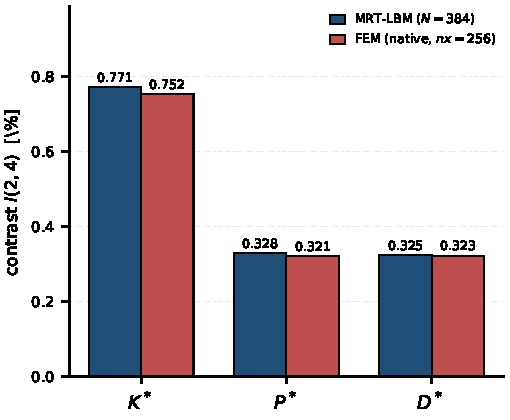
\includegraphics[width=0.75\columnwidth]{figures/fig10_fem_xcheck.pdf}
\caption{(Color online) Independent-solver cross-validation at $Re=400$, $\alpha=0$. Geometric contrast $I(2,4)$ of the kinetic energy $K^*$, lid power $P^*$, and viscous dissipation $D^*$, computed on the finest grids of each solver---MRT-LBM ($N=384$, left bars) and Taylor--Hood finite-element (native, $nx=ny=256$, right bars)---on the same superelliptic geometry. All three contrasts agree to within $0.02$ percentage point; the finite-element values use the native element-wise strain-rate, lid-power, and kinetic-energy integrals (Table~\ref{tab:femxcheck}).}
\label{fig:femxcheck}
\end{figure}

\begin{figure}[t]
\centering
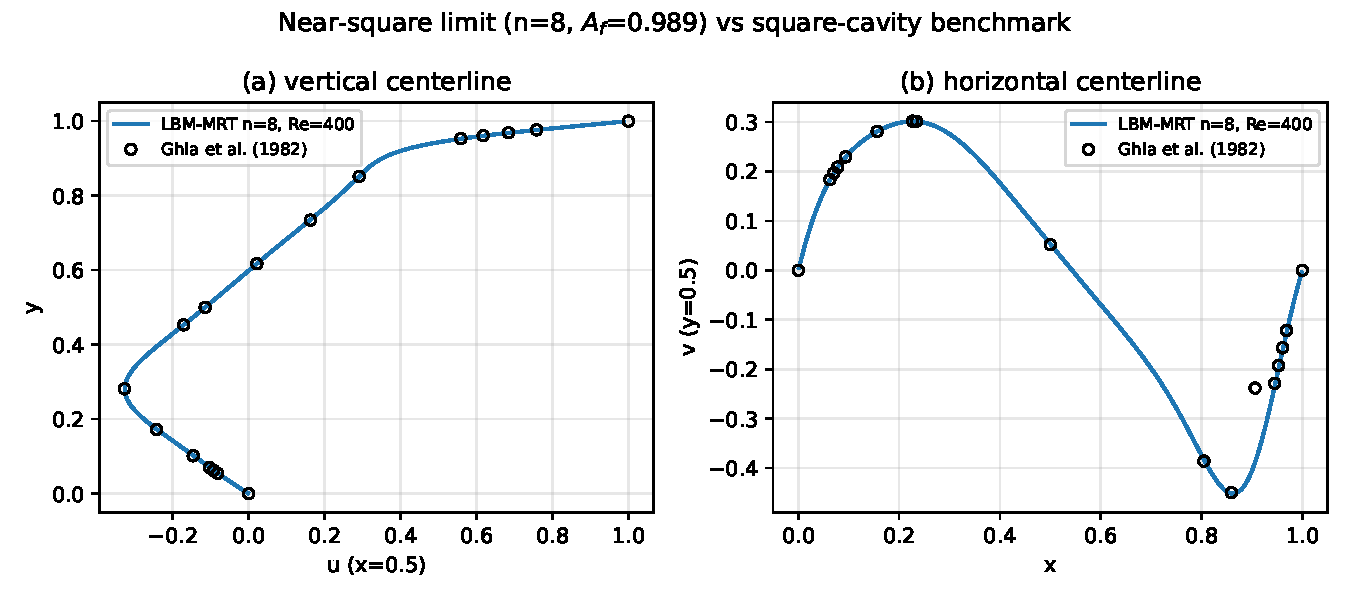
\includegraphics[width=0.9\columnwidth]{figures/fig2_benchmark.pdf}
\caption{(Color online) Near-square verification. Centerline velocity profiles of the $n=8$, $\alpha=0$ case at $Re=400$, $N=384$ (solid lines), compared with the square-cavity benchmark of Ghia et al.~\cite{Ghia1982} (open symbols). (a) Horizontal velocity $u$ along the vertical centerline $x=0.5$; (b) vertical velocity $v$ along the horizontal centerline $y=0.5$. The geometry is the closest available to the square limit ($A_f=0.9892$).}
\label{fig:benchmark}
\end{figure}

\begin{table}[t]
\centering
\caption{Exact square-cavity verification (flat bottom, uniform lid) against Ghia et al.~\cite{Ghia1982}. Maximum absolute deviations of the centerline velocity profiles at the tabulated interior reference stations: $\max|u-u_G|$ along the vertical centerline and $\max|v-v_G|$ along the horizontal centerline. The final column excludes the single anomalous tabulated datum at $(Re{=}400,\,x{=}0.9063)$~\cite{Chai2006}.}
\label{tab:ghia}
\small
\begin{tabular}{rrrrr}
\toprule
$Re$ & $N$ & $\max|u-u_G|$ & $\max|v-v_G|$ & $\max|v-v_G|$ (excl.) \\
\midrule
$100$  & $128$ & $0.0075$ & $0.0109$ & $0.0109$ \\
$100$  & $256$ & $0.0062$ & $0.0102$ & $0.0102$ \\
$400$  & $128$ & $0.0080$ & $0.1458$ & $0.0075$ \\
$400$  & $256$ & $0.0033$ & $0.1492$ & $0.0058$ \\
$1000$ & $128$ & $0.0120$ & $0.0107$ & $0.0107$ \\
$1000$ & $256$ & $0.0050$ & $0.0136$ & $0.0136$ \\
\bottomrule
\end{tabular}
\end{table}
\subsection{Resolution-sensitivity strategy}
\label{subsec:resolutionstrategy}

Three grid resolutions are employed: $N=128$, $256$, and $384$, corresponding to refinement factors of $2$ and $1.5$. These are chosen to bracket the finest resolution that can be afforded for the full parameter matrix within available compute resources, and to expose any non-monotonic behavior that a two-point comparison would miss. The refinement ratios are not uniform, and the residual change between the two finest grids is dominated by the partial cancellation of common discretization error rather than by a clean power-law decay; no Richardson extrapolation or grid-convergence index is therefore reported. Instead, the raw values at all three resolutions are reported and the span over $N=128$--$384$ is retained as a conservative numerical uncertainty (Section~\ref{subsec:robustness}). The language of ``resolution sensitivity'' is retained throughout; the term ``grid-independent solution'' is not used, since the data do not establish it to that standard.
